\graphicspath{{images/}}

In this section an evaluation of \mad on a real case-study is
presented, the commissioning of OpenStack. As in the previous section,
all results presented below can be reproduced by following the lab on
the following publicly available repository:
\footnote{\url{https://gitlab.inria.fr/VeRDi-project/madeus-journal/lab}}. First
this lab offers the possibility to reproduce the figures presented in
this section from the raw data obtained in our experiments on
Grid'5000. Second, the lab redraws the complete process to reproduce
the experiments on the Grid'5000 platform.

%------------------------------------
\subsection{OpenStack}
\label{subsec:openstack}
%------------------------------------

OpenStack is the de-facto open-source solution to address the IaaS
level of the Cloud paradigm, in other words OpenStack can be seen as
the open-source operating system of the Cloud. Since $2010$, its
community has gathered nearly $700$ organizations (such as Google, IBM
or Intel) and has produced more than $20$ million lines of code. Its
adoption is still growing in various domains such as public
administrations, e-commerce and science\footnote{See
  \url{http://superuser.openstack.org/} for further information.}.

OpenStack is a large distributed software system that brings together
almost $100$ software projects. Each project is in charge of a
specific aspect of the infrastructure management (\eg provision
virtual machines, provide them with storage, interconnect them through
networks), and their cooperation is the key to providing the features
required by Cloud management.
%
Those projects are themselves composed of several software modules
that are responsible for very specific tasks (\eg placement,
hypervisors etc.). While they are not all mandatory to deploy an
operable IaaS, $250$ software modules are available in those projects.
%
An OpenStack instance is a composition of some of those modules by the
operator. The chosen modules then cooperate to respond to the operator
requirements. For instance, the operator may need services to manage
virtual rather than bare-metal machines, object storage rather than
file-systems, while VLAN networks and billing services may not be
desired in her use-case. As defined in the large OpenStack
documentation, each software module has its own commissioning process,
and may depend on other modules commissionings.
%
The deployment of a typical OpenStack instance implies thus many
software modules whose commissioning process is characterized by a
large amount of tasks and interplays. As a consequence, the
commissioning process of OpenStack is complex to understand and can be
very long when tasks are executed sequentially.
%
In the following, we show how the commissioning process of an
OpenStack project can be transcribed as a \mad component. Leveraging
\mad enables us to express tasks and components coordination. As a
consequence, the \mad modeling improves the global commissioning
process understandability, and can be used to reduce commissioning
time by exploiting \emph{SIMH}, \emph{inter-comp}, \emph{inter-comp-tasks}
and \emph{intra-taks} parallelism levels.

\begin{table*}
  \begin{center}
    
\begin{tabular}{|c|c|c|c|c|}
   \hline
   & Roles & Places & Transitions & Ports \\
   \hline
   Nova & Manages compute instances (\eg Virtual machines) & 5 & 8 & 8\\
   Glance & Compute image store & 3 & 4 & 7\\
   Neutron & In charge of network resources & 3 & 4 & 7\\
   MariaDB & An SQL server used by most projects to store persistent
    information & 4 & 5 & 4\\
   Keystone & Manage user authentication, authorization and service
    discovery & 3 & 2 & 4\\
   RabbitMQ & The message bus for inter-service communication & 2 & 1 & 3\\
   HAProxy & Load-balances the requests to OpenStack controllers & 2 & 1 & 7\\
   OpenVSwitch & Virtualizes network functions & 3 & 1 & 2\\
   MemCached & Caches ephemeral data for most OpenStack projects & 2 & 1 & 2\\
   Facts & Collects informations about every nodes & 2 & 1 & 1\\
   Common & Common utilities (\eg cron, fluentd: a metric collector for logging)
    & 3 & 2 & 2\\
%   \hline
%   Total & 32 & 30 & 47 & \\
%   \hline
%   & Places & Transitions & Ports & Roles\\
%   \hline
%   Nova & 5 & 8 & 8 & Manage compute instances (\eg Virtual machines)\\
%   Glance & 3 & 4 & 7 & Compute image store\\
%   Neutron & 3 & 4 & 7 & In charge of network resources\\
%   Keystone & 3 & 2 & 4 & Manage user authentication, authorization and service
%    discovery\\
%   MariaDB & 4 & 5 & 4 & An SQL server used by most projects to store persistant
%    information\\
%   RabbitMQ & 2 & 1 & 3 & The message bus for inter-service communication\\
%   HAProxy & 2 & 1 & 7 & Load-balances the requests to OpenStack API services\\
%   OpenVSwitch & 3 & 1 & 2 & Virtualizes network functions\\
%   MemCached & 2 & 1 & 2 & Caches ephemeral data for most OpenStack projects\\
%   Facts & 2 & 1 & 1 & Collects inforamtions about every nodes\\
%   Common & 3 & 2 & 2 & Common utilities (\eg cron, fluentd: a
%   metric collector for logging) \\
   \hline
   Total & & 32 & 30 & 47\\
   \hline
\end{tabular}


    \caption{Number of places, transitions, ports and roles for each \mad component
        of the OpenStack assembly of Figure~\ref{fig:full}.}
    \label{tab:os}
  \end{center}
\end{table*}

\HC[Dimitri]{verifier phrase out-of-the-box}

\kolla is one of the most popular tool for deploying OpenStack in
production.  It relies on \ansible to deploy OpenStack's modules as
\docker containers, and will be considered as our reference in the
rest of this section. It is highly opinionated out-of-the-box,
allowing operators to quickly deploy a basic OpenStack instance, but
not enabling the complete customization for advanced
administrators. As a consequence, the use-case described in this
section corresponds to the default \kolla deployment, which provides
the essential mechanisms to operate an infrastructure with OpenStack.
%
To compare the performance of \kolla and \mad, we have defined $11$
\mad components based on the \ansible roles defined in \kolla's
playbooks (\ie \ansible sequence of components to comission). Their
names are built for most of them on the OpenStack project they deploy.
\Cref{tab:os} lists these components and indicates which aspect of the
Cloud management they are in charge of. Furthermore, some \mad metrics
are displayed (\ie the number of places, transitions and ports).
%
In this table, when the number of transitions is greater than the
number of places plus one, it means that \mad can be leveraged to
express parallel transitions. Also, the more ports, the more \mad have
to coordinate interplays during the commissioning. As depicted in
\cref{tab:os}, Nova, Glance, Neutron and MariaDB are components of
particular interests since they contain more transitions and ports
than the others.

%------------------------------------
\subsection{Expressivity and Separation of Concerns}
%------------------------------------

\begin{figure*}
  \begin{center}
    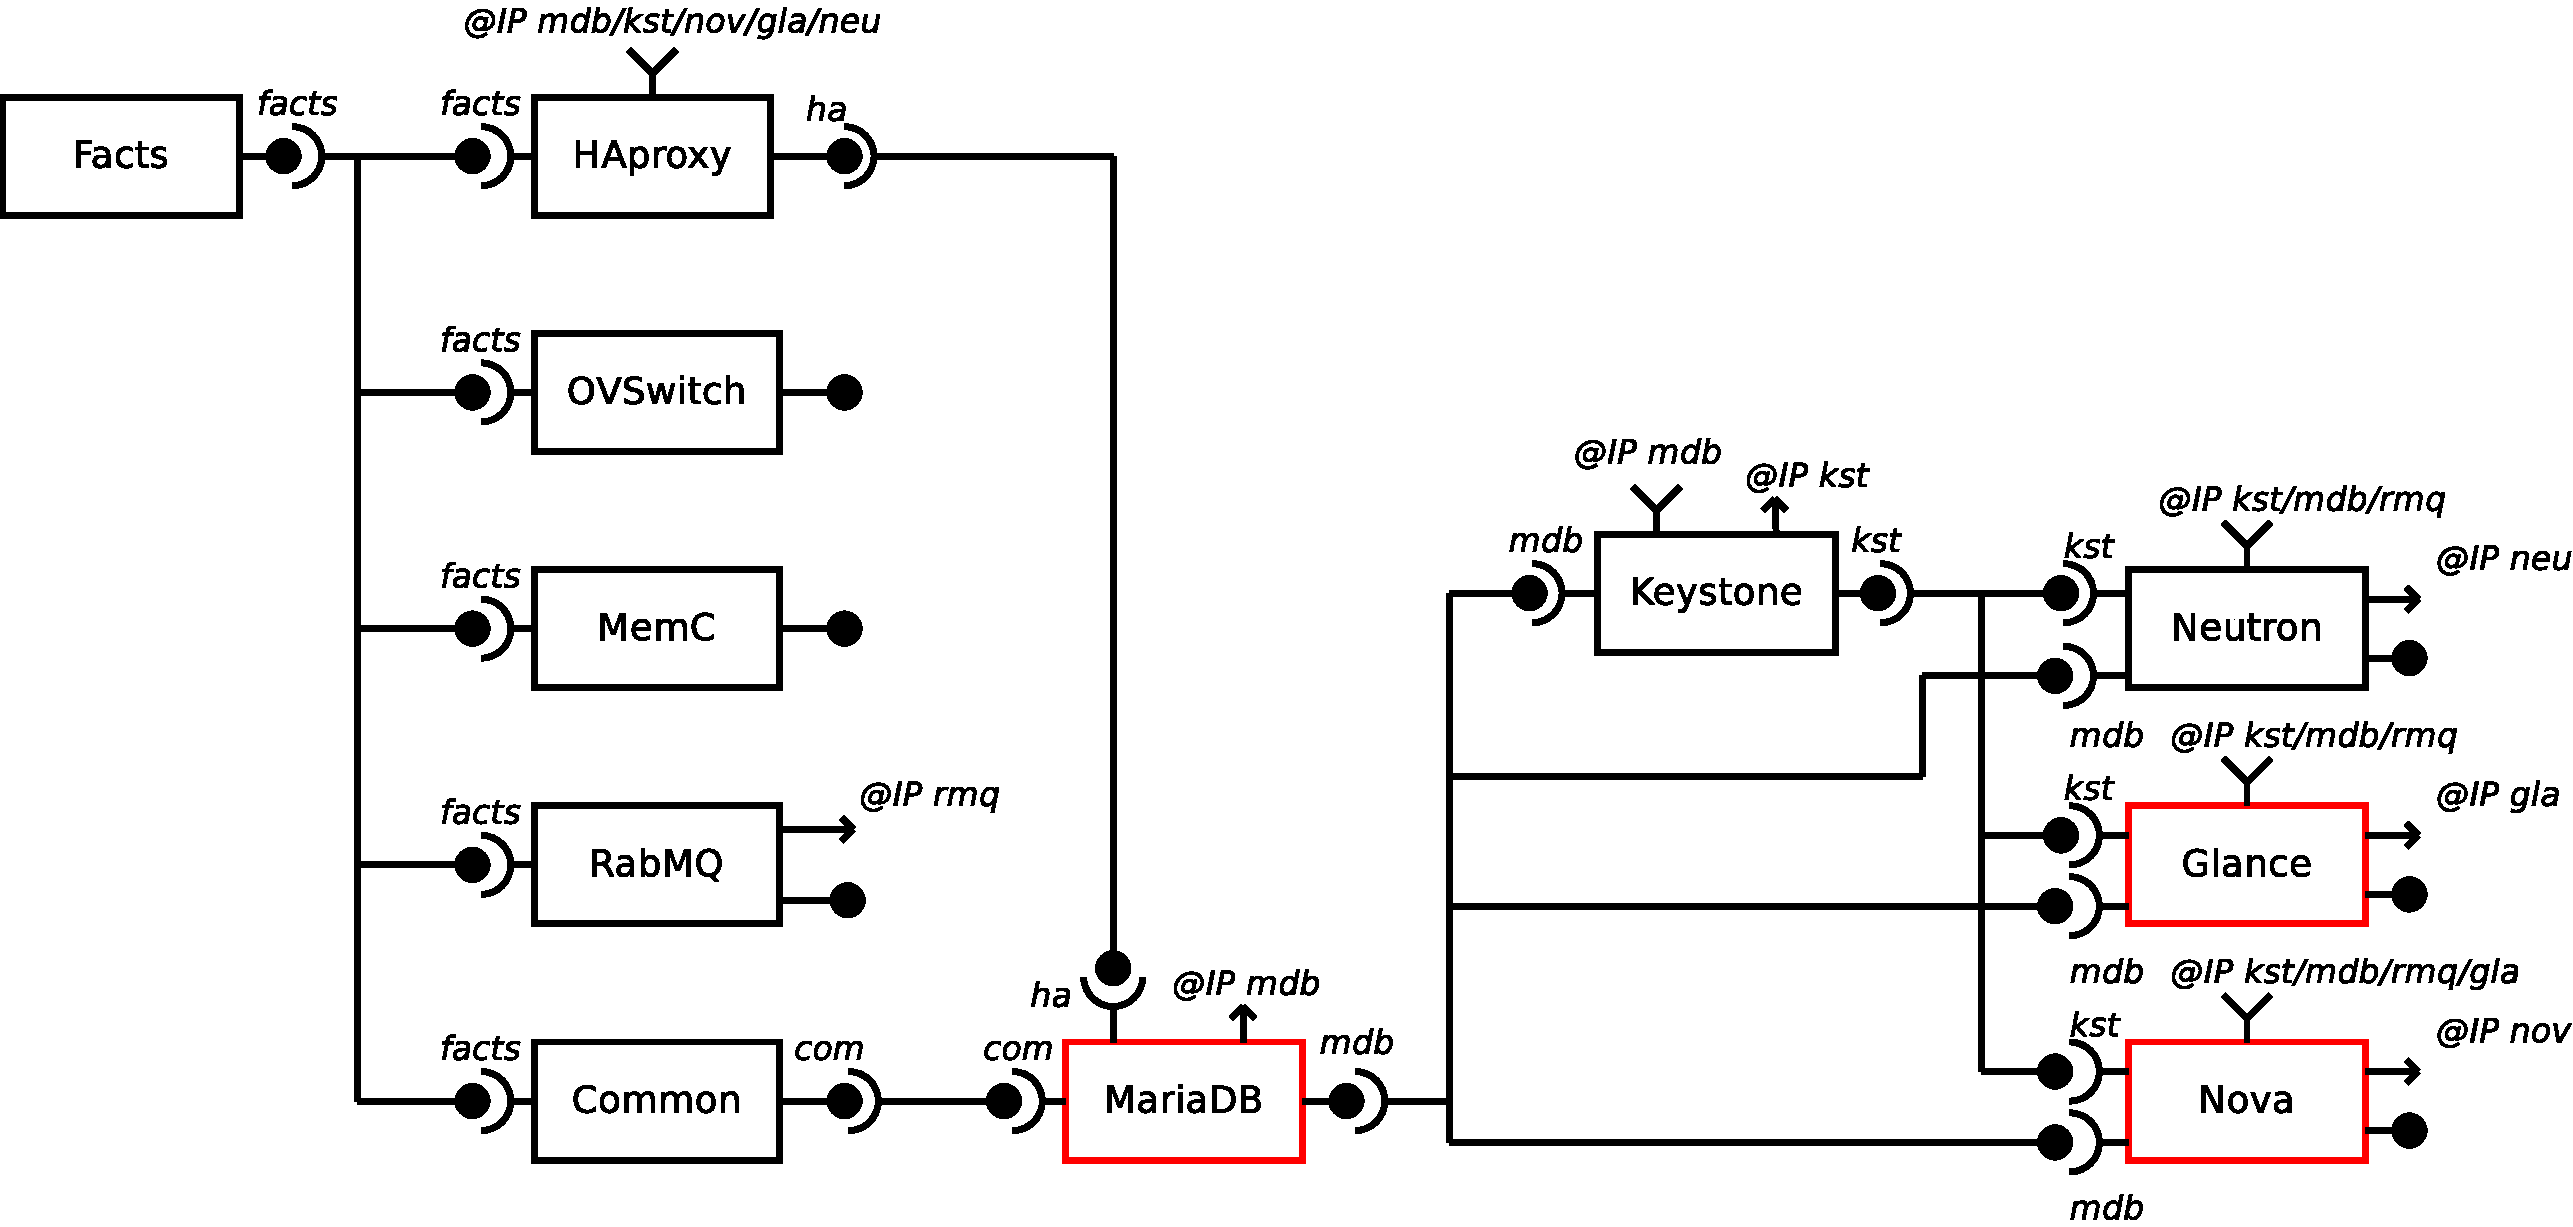
\includegraphics[width=0.7\textwidth]{./images/full.pdf}
    \caption{Simplified \mad assembly of the \kolla-based OpenStack deployment
    containing $11$ components. Connections between data ports are not depicted.
    Red components are detailed in \cref{fig:sub}.}
    \label{fig:full}
  \end{center}
\end{figure*}

Figure~\ref{fig:full} depicts the use-case from the operator viewpoint (\ie
at the level of the \mad assembly). For the sake of simplicity and
readability, the connections between data ports are not
represented. This figure helps to understand the high-level of
interplays between components. For instance, Neutron, Glance and Nova
require Keystone, while Keystone requires itself a database (\ie
MariaDB) for its commissioning process. Regarding the separation of
concerns, the operator does not need to understand component
internals. She just needs to compose the desired components by listing
them and connecting their compatible ports. As a consequence, a
component can be replaced by another one if they expose the same
interfaces. For instance the operator could replace MariaDB with
MySQL: another component which also implements a database by exposing
the same ports.

\begin{figure*}[t]
  \begin{center}
    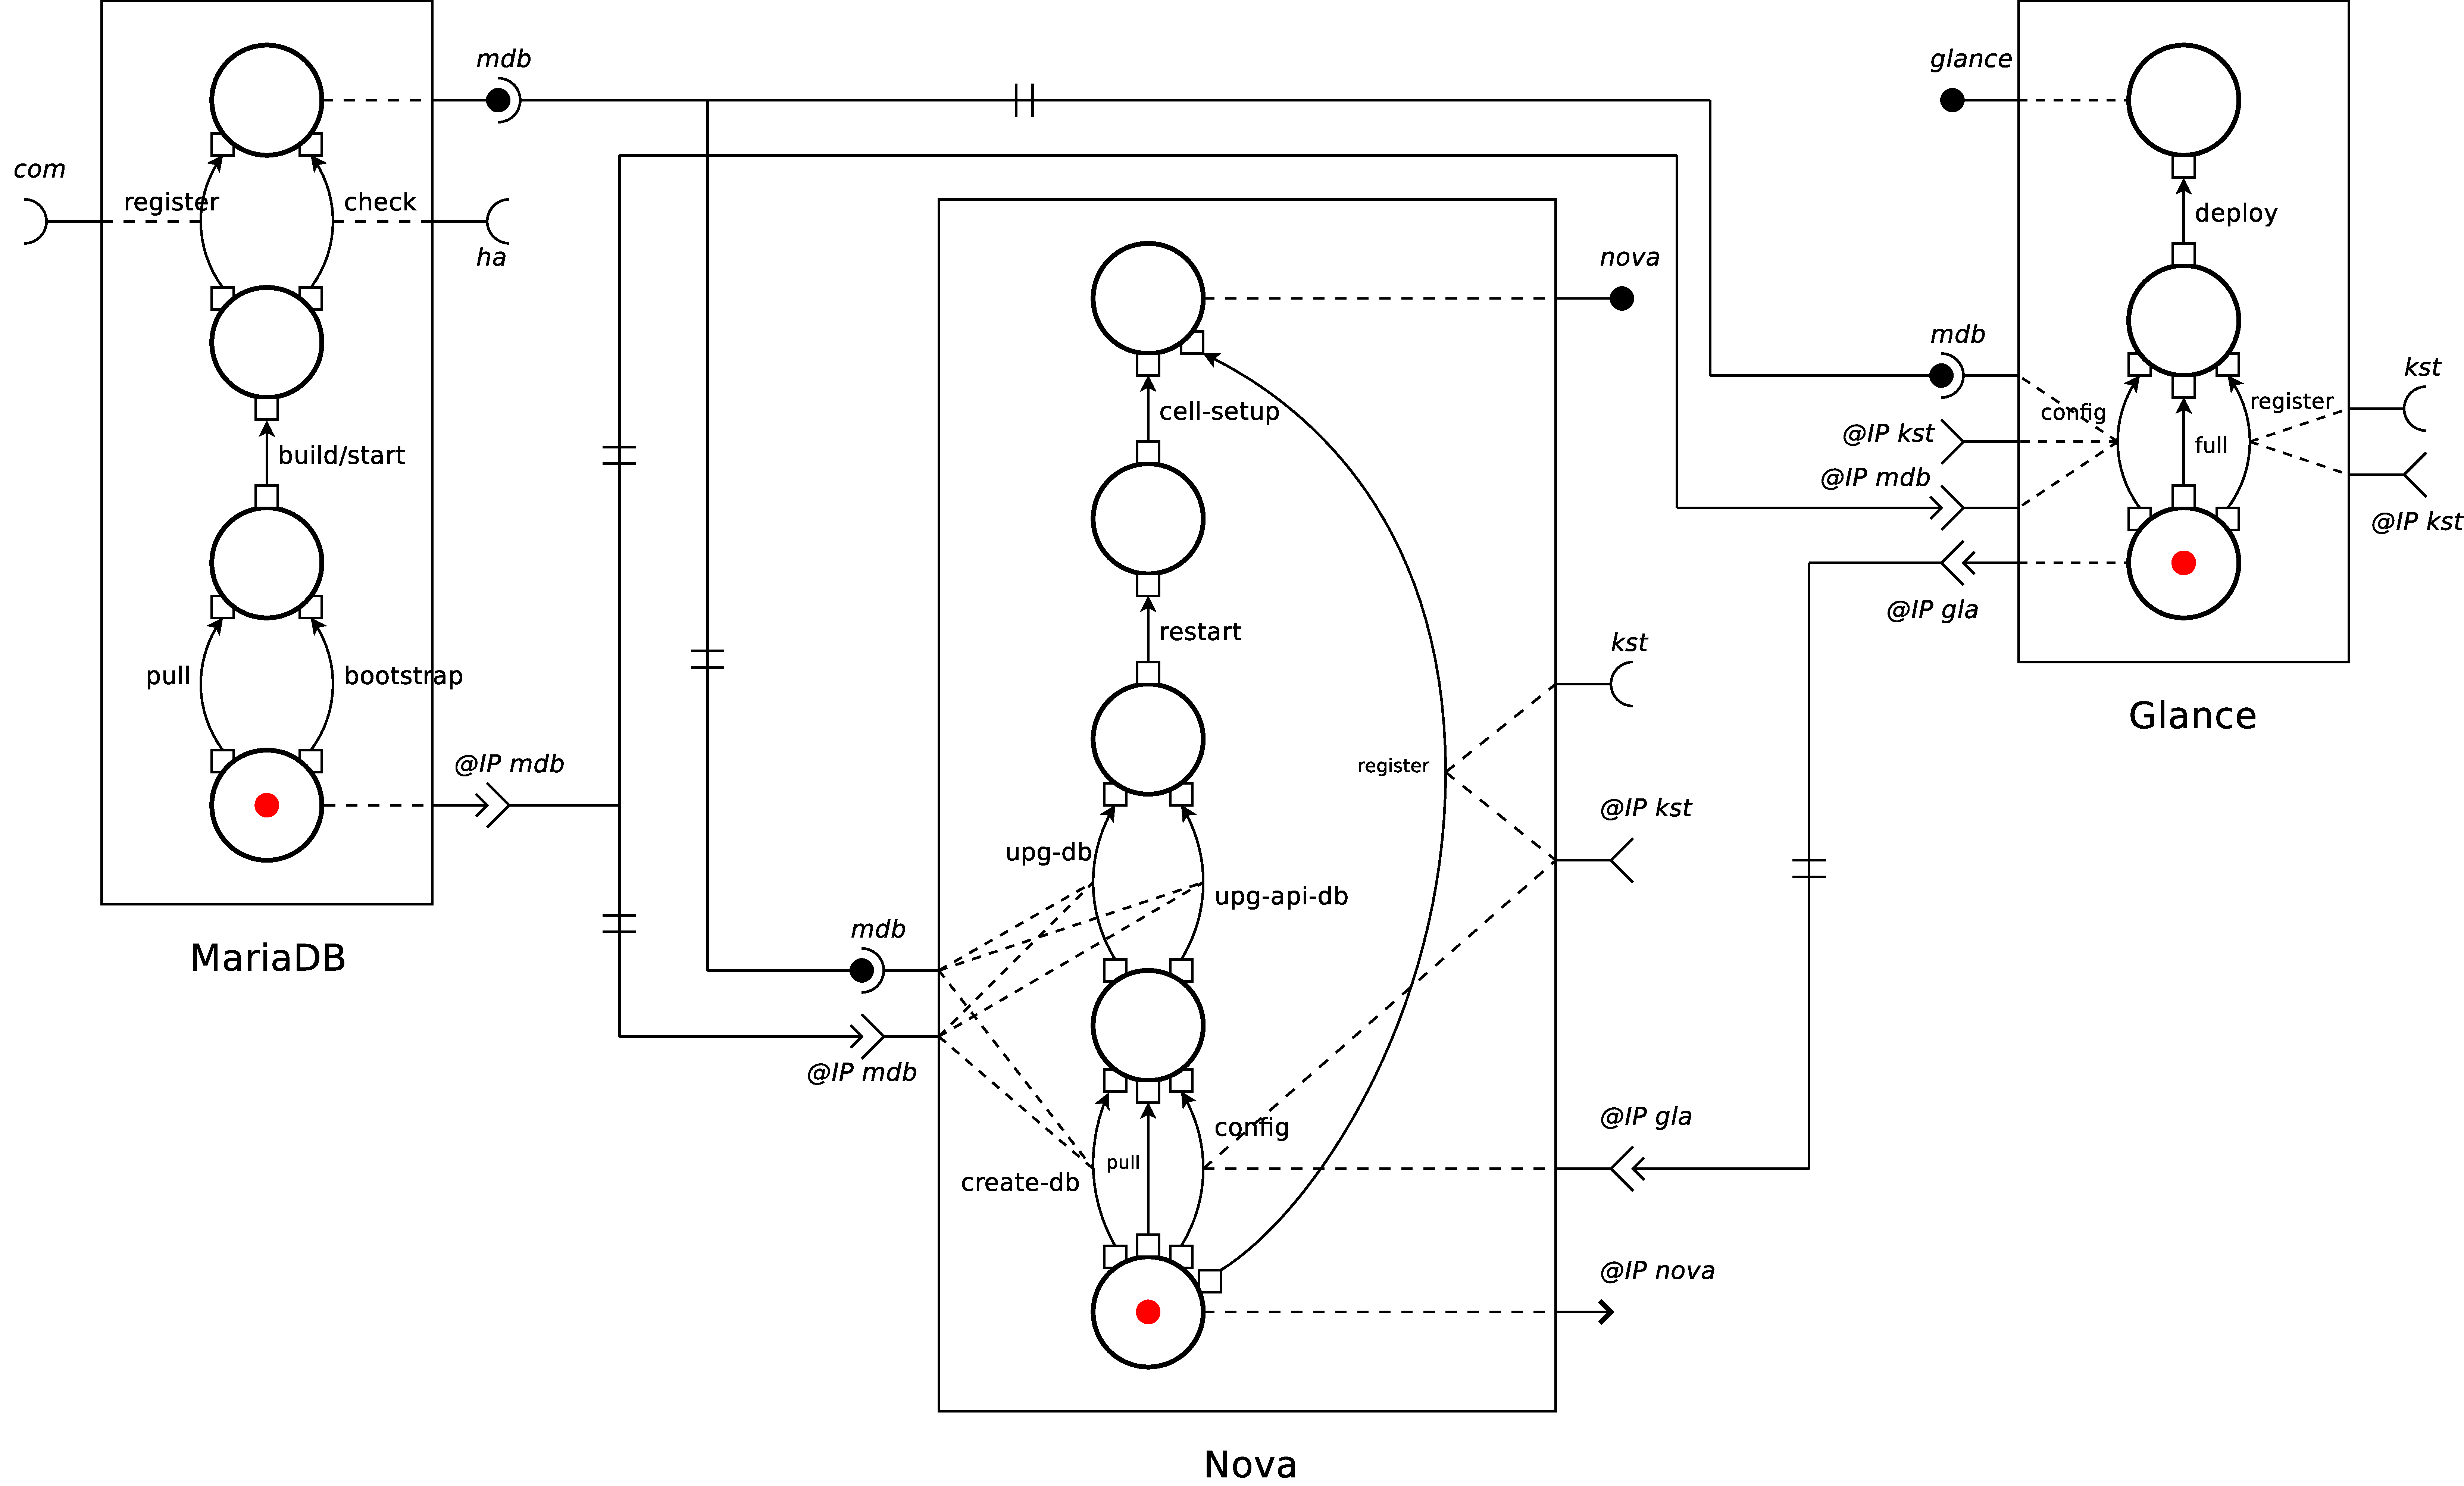
\includegraphics[width=0.8\textwidth]{./images/sub.pdf}
    \caption{A detailed sub-part of the previous component assembly to deploy
    OpenStack.}
    \label{fig:sub}
  \end{center}
\end{figure*}
%TODO: J'aurais peut être représenté Keystone à la place de MariaDB
%   1. Est-ce utile de dire que mariadb ici est différent de mariadb avant et
%   pas risqué pour embrouiller le message ?
%   2. Register est une transition liée à Keystone qui est très intéressante
%   quand on examine Nova (transition indépendante des autres)

We now study our use-case from the developer viewpoint, focusing on
the three colored components from Figure~\ref{fig:full}: MariaDB, Nova and
Glance. Figure~\ref{fig:sub} depicts the internals and interplays of these
components.

The dependencies previously observed at the assembly level are more
detailed at the developer level. First, if we isolate Nova and Glance
for instance, while Figure~\ref{fig:full} let us think that Glance
must be deployed before Nova, it is clear here that once Nova obtains
Glance's IP address (provided by the first place in Glance), both
components can be deployed in parallel. This shows how \mad can be
leveraged for \emph{inter-comp} and \emph{inter-comp-tasks}
parallelism.  Second, as we discussed before, it seemed in
Figure~\ref{fig:full} that MariaDB must be deployed before Keystone,
and Keystone before Neutron/Glance/Nova. However, with the \mad
representation depicted in Figure~\ref{fig:sub}, we understand that
only the \emph{register} transition of Glance and Nova requires the
service catalog Keystone to be available (\ie to register themselves
in the catalog). We can see on the figure that other tasks can be
executed in parallel while \emph{register} waits for Keystone (\eg for
Nova, this transition is independent for all the other
ones). Similarly, Figure~\ref{fig:sub} depicts for each component many
parallel transitions showing how \mad can be leveraged for
\emph{intra-comp-tasks} parallelism in this use-case.

%------------------------------------
\subsection{Experimental Setup and Parameters}
% ------------------------------------

This section defines first the experimental setup: (i) how modules are
distributed among nodes (\ie servers or machines) and (ii) the testbed
characteristics. Then we describe the different parameters used during
our experimentation: (iii) the assemblies we designed to compare our
contribution with the related work and (iv) the way \docker images are
fetched by nodes.

%-------
\paragraph{Node roles and module distribution}
Each of the $11$ components defined earlier in \kolla is in charge of
an OpenStack project. As we said previously, each OpenStack project
contains multiples software modules. Hence, each component actually
deploys different modules ($36$ in total). A basic multi-node \kolla
deployment targets three nodes. First, the \emph{Control} node, which
hosts control services, APIs and databases, commissioning $16$
services. The second one is the \emph{Network} node that hosts network
agents and HAProxy, and contains $11$ services. Finally, the
\emph{Compute} node, in charge of compute services and VMs placement,
hosts $9$ services.

\begin{table}
  \begin{center}
    \small
    
\begin{tabular}{|c|c|c|c|}
   \hline
   Cluster & CPU & Memory & Network\\
   \hline
   Nova & 2 x Intel Xeon E5-2620 v4 & 64GB & 10Gbps\\
   (lyon) & 8 cores/CPU &  & \\
   \hline
   Taurus & 2 x Intel Xeon E5-2630 & 32GB & 10Gbps\\
   (lyon) & 6 cores/CPU & & \\
   \hline
   Sol & 2 x AMD Opteron 2218 & 4GB & 1Gbps\\
   (sophia) & 2 cores/CPU & &\\
   \hline
\end{tabular}


    \caption{Grid'5000 cluster configurations.}
    \label{tab:g5k}
  \end{center}
\end{table}

%-------
\paragraph{Testbed and resource provisioning}
Our evaluations have been conducted on two clusters from the
experimental platform Grid'5000: \ecotype and \nova. \Cref{tab:g5k}
shows the hardware configuration for both clusters. The cluster
\ecotype has a better hardware configuration than the latter,
regarding CPU, memory and network interfaces, as detailed in the
table. To design reproducible benchmarks, we used
EnosLib\footnote{\url{https://gitlab.inria.fr/discovery/enoslib}}, a
library to build experimental frameworks on multiple testbeds (\eg
Grid5000, LibVirt), and
Execo\footnote{\url{http://execo.gforge.inria.fr/doc/latest-stable/index.html}},
another library for prototyping experiments. Since \kolla, our
reference, does not manage resource provisioning, we do not include
this phase in the use-case, nor in our benchmark. Even if resource
provisioning could be managed by \mad, this step is left to EnosLib
and not counted in execution times.

%-------
\paragraph{Assemblies}
Our performance evaluation compares three different assemblies that
are designed to capture the behavior of \ansible, \aeolus and \mad. To
that end, the component internals for each assembly vary with regards
to the number of places, transitions and ports. It is also important
to understand that we re-used the \ansible files already provided by
\kolla by splitting them into component transitions. By using \mad to
coordinate \ansible execution, it is possible for us to provide a way
to fairly compare these solutions. Moreover, by using splitted \kolla
roles the \emph{SIMH} parallelism level is handled by \ansible in the
three assemblies.

The first assembly, called \ansass matches the \kolla-ansible
commissioning process. Each component is triggered sequentially, in
the same way and order as \ansible triggers sequentially the roles
defined in \kolla. Since there is simply a sequential coordination
between components, their internals are composed of two states
connected by a single transition which performs all the commissioning
tasks, such as in \kolla (\ie no \emph{intra-comp-tasks}
parallelism). Each time a component is deployed, it activates the
commissioning process of the next one (\ie neither \emph{inter-comp}
nor \emph{inter-comp-tasks} parallelism). This assembly features the
first level of parallelism which is managed by \ansible when tasks are
mapped to multiple nodes, \ie \emph{SIMH} parallelism.
%

The second assembly, called \aeoass is equivalent to an \aeolus
commissioning of OpenStack. It provides parallelism at both the
\emph{inter-comp} and \emph{inter-comp-tasks} levels in addition to
\emph{SIMH}, and no \emph{intra-comp-tasks} parallelism. Coordination
is driven by component's ports. In this assembly, most components are
built with two sequential transitions. When the assembly is
initiated, the first transition of those components are triggered,
while the second one is conditioned by a dependency from another
component.
%

The third assembly, called \madass, leverages our contribution to
commission OpenStack. It corresponds to the one we previously
described when presenting the use-case. All the components have their
own internals definition, based on our understanding of the OpenStack
commissioning process. As depicted previously in \cref{tab:os}, most
components are built on multiple places and transitions. This assembly
relies on \mad to handle the four parallelism levels.

\begin{table}
  \begin{center}
    
\begin{tabular}{|c|c|c|c|}
   \hline
   & Compute & Network & Control\\
   \hline
   Number of images & $9$ & $11$ & $16$\\
   \hline
   Total Size (MB) & $2767$ & $2705$ & $4916$\\
   \hline
\end{tabular}


    \caption{Number of \docker images per node and their cumulated size in MB to
      download from the registry.}
    \label{tab:images}
  \end{center}
\end{table}

%-------
\paragraph{Docker container registry}
Finally, since \kolla relies on \docker containers, fetching \docker
images has a significant impact on our results: images have to be
downloaded, before being decompressed. To be as neutral as possible we
have conducted experiments with three different modes for handling
those images: (1) \emph{cached} mode, where images are previously
placed on OpenStack nodes, so fetching \docker images has no impact on
the results; (2) \emph{local} mode, where images are previously
downloaded on a new dedicated node of the cluster, from which images
can be loaded (\ie a local \docker registry); (3) \emph{remote} mode,
in which images are fetched from an Internet repository (\ie the
DockerHub registry). \Cref{tab:images} gives for each OpenStack node
(\ie Compute, Network and Control) the number of \docker images to
download and their compressed size.  As depicted in this table, more
than $10$GB must be downloaded in our use-case.  Furthermore, the
control node has to download almost twice as much data than the other
nodes.

%------------------------------------
\subsection{Results}
%------------------------------------

In this section, we analyze the results of our benchmark through
different aspects: (i) the performance of each assemblies; (ii) the
adequation between the theoretical predicted performance and the
observed results and (iii) the influence of registry modes on our
results.

\begin{figure}[t!]
  \begin{center}
    \def\svgwidth{\columnwidth}
    \subfloat[Performance comparison on \ecotype]{
      \input{./images/use_case_ecotype_perf.pdf_tex}
      \label{fig:ecotype}
    }
    \def\svgwidth{\columnwidth}
    \subfloat[Performance comparison on \nova]{
      \input{./images/use_case_nova_perf.pdf_tex}
      \label{fig:nova}
    }
    \caption{Recorded time in seconds for OpenStack commissioning with
      different clusters, assemblies and registry modes. Upper parts
      represent mean values with relative ratios for each result
      compared to the reference \ansass.  Lower parts display means,
      standard deviations and the minimum and maximum values computed
      from the theoretical performance model, depicted as boxes.}
    \label{fig:openstack_results}
  \end{center}
\end{figure}

\begin{table}
    \begin{center}
        
\begin{tabular}{cll|ccc}
\toprule
& & & remote & local & cached  \\

\midrule
\multirow{9}{*}{\STAB{\rotatebox[origin=c]{90}{measured}}} & \multirow{3}{*}{\STAB{\rotatebox[origin=c]{90}{mean}}}  & ansible  &
530s  &
480s  &
331s  \\
  & & aeolus  &
263s  &
256s  &
229s  \\
  & & madeus  &
152s  &
148s  &
128s  \\
\cmidrule{2-6}& \multirow{3}{*}{\STAB{\rotatebox[origin=c]{90}{gain}}}  & ansible  &
0\%  &
0\%  &
0\%  \\
  & & aeolus  &
50\%  &
46\%  &
30\%  \\
  & & madeus  &
71\%  &
69\%  &
61\%  \\
\cmidrule{2-6}& \multirow{3}{*}{\STAB{\rotatebox[origin=c]{90}{std}}}  & ansible  &
1s  &
1s  &
0s  \\
  & & aeolus  &
2s  &
1s  &
1s  \\
  & & madeus  &
4s  &
4s  &
3s  \\
\midrule
\multirow{6}{*}{\STAB{\rotatebox[origin=c]{90}{theoretical}}} & \multirow{3}{*}{\STAB{\rotatebox[origin=c]{90}{max}}}  & ansible  &
540s  &
485s  &
334s  \\
  & & aeolus  &
269s  &
259s  &
232s  \\
  & & madeus  &
156s  &
158s  &
136s  \\
\cmidrule{2-6}& \multirow{3}{*}{\STAB{\rotatebox[origin=c]{90}{min}}}  & ansible  &
523s  &
473s  &
326s  \\
  & & aeolus  &
257s  &
249s  &
223s  \\
  & & madeus  &
141s  &
143s  &
123s  \\
\bottomrule
\end{tabular}

        \caption{Measured and theoretical results of our benchmark on \ecotype.}
        \label{tab:openstack_results}
    \end{center}
\end{table}

In these different studies, we will refer to
Figures~\ref{fig:ecotype,fig:nova} which respectively show our results
on \ecotype and \nova clusters. The upper part displays the recorded
times to commission OpenStack as a function of the three different
assemblies studied. For a better understanding of the comparison, the
value of each result is written on top of the bars, while the ratio
compared to \ansass, our reference, is displayed below the bars'
edges.  Furthermore, for each assembly on the X-axis, the results for
the three \docker registry settings are displayed with different
colors: blue, red and green respectively for \emph{remote},
\emph{local} and \emph{cached} respectively. On the lower part, the
means for each result are depicted as blue, red and green horizontal
lines, the related standard deviations are represented by vertical
lines, while boxes represent the minimum and maximum values computed
with the theoretical performance model of
Section~\ref{sec:perf_model}.
% 
For the sake of readability, the scale of the lower parts are
differents for each assembly. Each result corresponds to the average
computed from $10$ iterations. The corresponding numerical values are
also displayed in \cref{tab:openstack_results}.
%
\HC[Dimitri]{pourquoi les resultats sur ecotype seulement dans le
  tableau? mettre 2 tableaux?}
% Et bien ça en fait un beau paragraphe pour seulement expliquer comment
% fonctionne la figure ^^'...

%-------
\paragraph{Impact of assemblies}

\begin{figure*}[t]
  \begin{center}
    %\vspace{-3em}
    \def\svgwidth{\columnwidth}
    \scriptsize
    \subfloat[\ansass with \emph{cached} registry]{
      \scalebox{0.9}{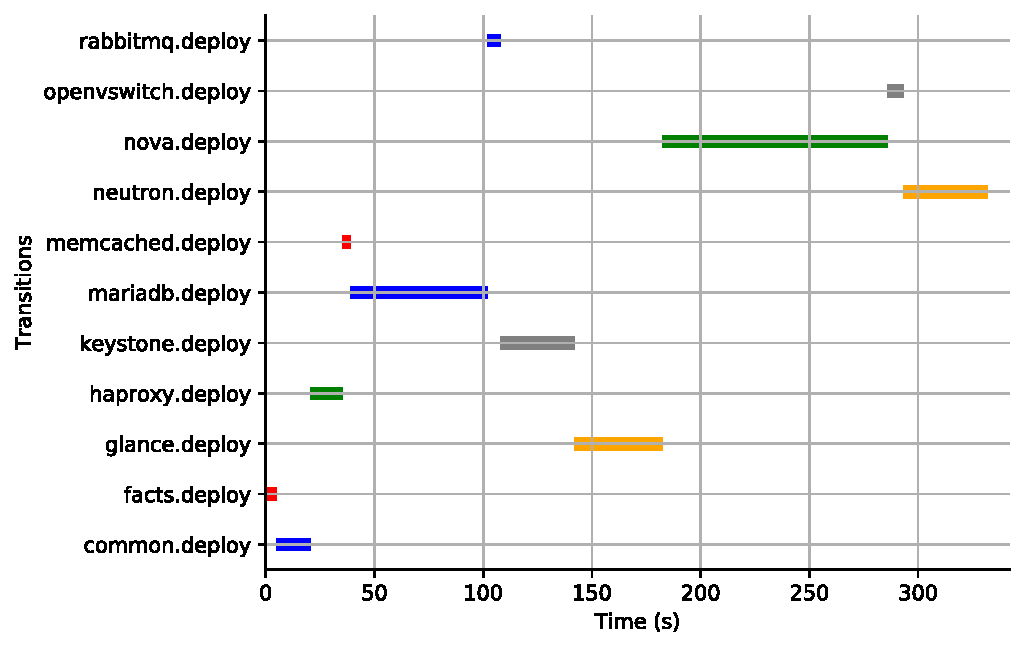
\includegraphics[scale=0.5]{./images/use_case_gantt_cached_ansible.pdf}}
      \label{fig:gantt_ansible}
    }
    %\vspace{-3em}
    \def\svgwidth{\columnwidth}
    \scriptsize
    \subfloat[\aeoass with \emph{cached} registry]{
      \scalebox{0.9}{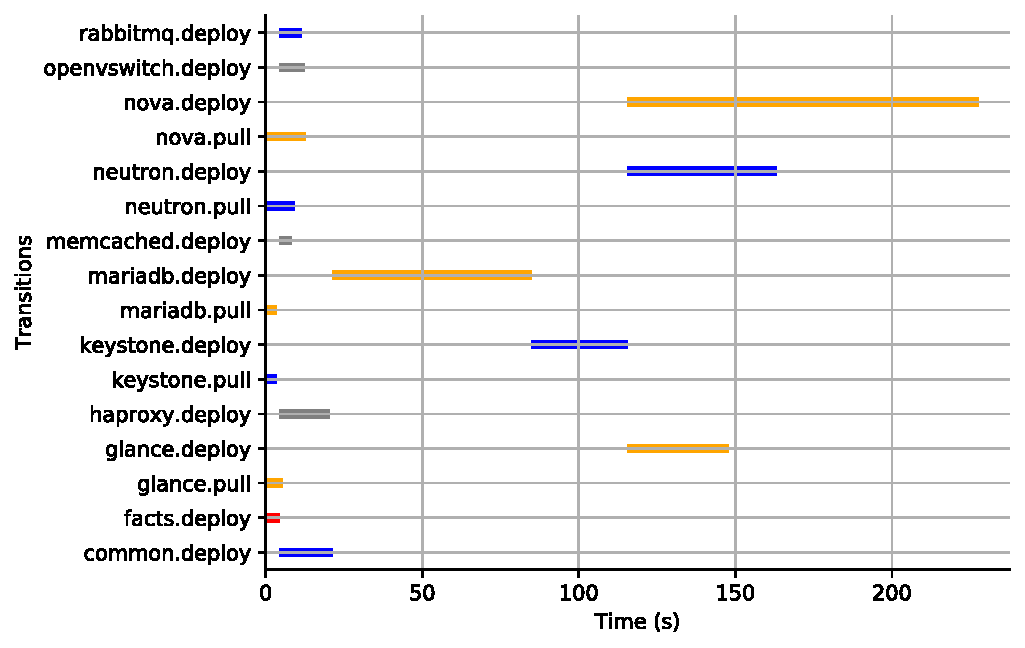
\includegraphics[scale=0.5]{./images/use_case_gantt_cached_aeolus.pdf}}
      \label{fig:gantt_aeolus}
    }
    %\vspace{-3em}
    \def\svgwidth{\columnwidth}
    \tiny
    \subfloat[\madass with \emph{cached} registry]{
      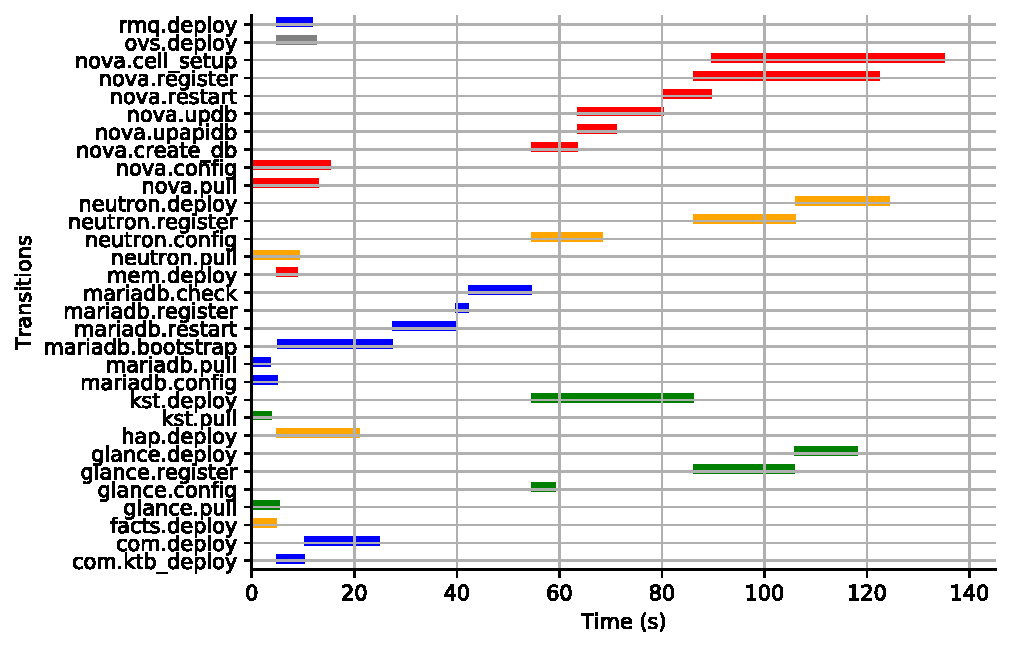
\includegraphics[scale=0.5]{./images/use_case_gantt_cached_mad.pdf}
      \label{fig:gantt_madeus}
    }
    \def\svgwidth{\columnwidth}
    \tiny
    \subfloat[\aeoass with \emph{remote} registry]{
      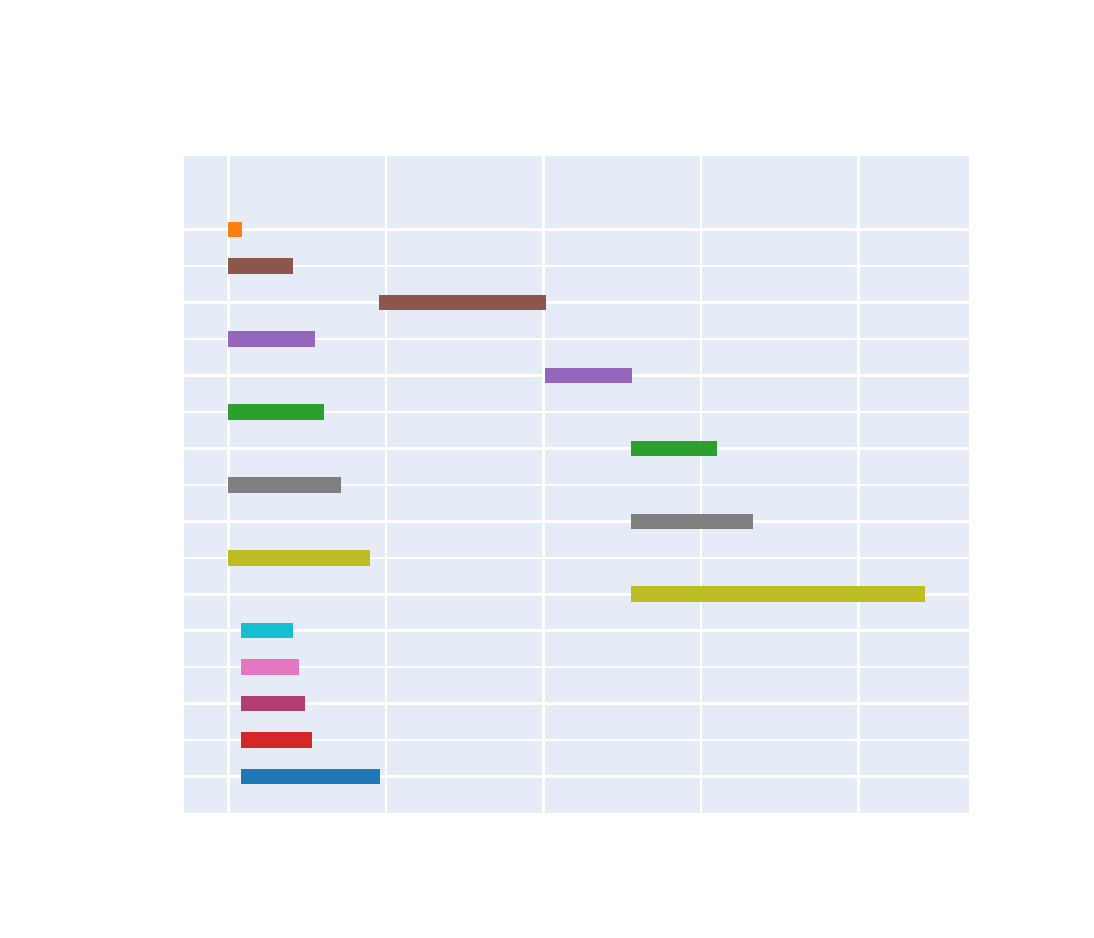
\includegraphics[scale=0.5]{./images/use_case_gantt_remote_aeolus.pdf}
      \label{fig:gantt_aeolus_remote}
    }
    \caption{(a), (b) and (c) Gantt charts of the OpenStack
      commissioning for the three different assemblies with the
      registry set in \emph{cached}; (d) Gantt chart of the OpenStack
      commissioning for \aeoass, with the registry set in
      \emph{remote}.}
  \end{center}
\end{figure*}

We now compare the time measured to commission OpenStack regarding the
three assemblies defined previously: \ansass, \aeoass and \madass (the
lower, the better in Figure~\ref{fig:openstack_results}).  As
expected, the time required to commission these assemblies reflects
the level of parallelism they handle. Since \ansass is limited to the
first parallelism level, \ie \emph{SIMH}, its commissioning time is
longer than \aeoass. By featuring \emph{inter-comp} and
\emph{inter-comp-tasks} parallelism, the latter outperforms the former
from $26$\% (\nova, \emph{cached}) to $50$\% (\ecotype,
\emph{remote}). Leveraging \emph{intra-comp-tasks} parallelism enables
\madass to outperform \ansass~from $45$\% (\nova, \emph{cached}) to
$71$\% (\ecotype, \emph{remote}), and \aeoass from $16$\% (\nova,
\emph{remote}/\emph{local}) to $30$\% (\ecotype, \emph{cached}). As a
result, considering the maximum gain compared to \ansass on \ecotype
the OpenStack commissioning goes from almost 9 minutes to less than 3
minutes.
%
\HC[Dimitri]{Ajouter un paragraphe sur l'application à OpenStack-CI,
  comment on a fait les requetes et quel gain ca donnerait sur 24h}

To go further in this analysis, we propose to analyze the
commissioning process at the level of transitions (\ie tasks). To
investigate this aspect, we implemented in \mad the ability to
generate Gantt charts that display the execution time of the different
transitions for each component.
% Maybe something to put in the implementation part
Figures~\ref{fig:gantt_ansible,fig:gantt_aeolus,fig:gantt_madeus}
respectively represent the Gantt charts of the commissioning execution
of \ansass, \aeoass and \madass, when the registry is set to
\emph{cached} on \ecotype. Each line of these figures represents a
transition as a function of the elapsed-time displayed on the X-axis.
First, as previously explained, Figure~\ref{fig:gantt_ansible} shows that a
single transition exists in each component of the \ansass
assembly. Thus, here, each line also corresponds to one component
commissioning. As expected, the figure shows that each component is
deployed in a sequential way. The first level of parallelism (\ie
\emph{SIMH}) is not visible in these figures since it is handled
internally by \ansible playbooks executed in each transition of the
assembly. One can note that Nova, MariaDB, Glance, Keystone and
Neutron are particularly long to commission. \aeoass and \madass
accelerate the process by combining (i) splitting the transition of
components into smaller ones and (ii) managing more or less
dependencies between them (depending on the ability to express
\emph{inter-comp}, \emph{inter-comp-tasks} and \emph{intra-comp-tasks}
parallelism).
%
Figure~\ref{fig:gantt_aeolus} illustrates that the components we
highlighted previously (\eg Nova in yellow, Neutron in gray) are based
on two transitions in \aeoass. This figure shows that this assembly
can leverage both the \emph{inter-comp} and \emph{inter-comp-tasks}
parallelism levels since we can see that multiple components and
different tasks of these components (\eg \texttt{glance.pull} and
\texttt{haproxy.deploy}) are executed in parallel. As a consequence,
the commissioning time drops from $5$ minutes and $31$ seconds to $3$
minutes and $49$ seconds.
%
Finally, Figure~\ref{fig:gantt_madeus} clearly shows how \mad
leverages the fourth level of parallelism (\ie \emph{intra-comp-tasks}
parallelism) by displaying multiple transitions executed in
parallel. For instance, transitions \texttt{nova.pull} and
\texttt{nova.config} (depicted in yellow), are performed
simultaneously which is not possible with \ansible or \aeolus. Hence
the commissioning time drops from $5$ minutes and $31$ seconds to $2$
minutes and $8$ seconds.
%

%-------
\paragraph{Precision of the performance model}
% Construire un tableau contenant les valeurs min/max/moy_obs/moy_calc
The maximum and minimum values obtained by the performance model described
previously is depicted in \cref{tab:openstack_results}. When analyzing these
results, one can first note that the measured mean is always between the
expected maximum and minimum. Secondly, the difference between the computed
maximum and minimum values is only from $2\%$ to $10\%$ the maximum value. As a
consequence, this validates the precision of our performance model.
This one can thus be used to detect anomalies in the component design
phase.
\HC[Dimitri]{better explanation - how is computed the min and max with
  which reference times? explain why it is a good estimation}

% donner un exemple ici - peut être développé précedemment dans la partie modèle
% de performance, ou intro pour motiver la contribution du modèle de perf ?

%-------
\paragraph{Influence of registry modes}

\begin{table}
  \begin{center}
    \begin{tabular}{lccc}
      \toprule
      & cached & local & remote\\
      \midrule
      \emph{pull}(s) & 9 & 78 & 127\\
      \emph{pull}(\%) & 3\% & 20\% & 32\%\\
      \bottomrule
    \end{tabular}
    \caption{Time spent in the \emph{pull} transition from Nova and
    percentage compared to the total time for \ansass commissioning.}
    \label{tab:pull}
  \end{center}
\end{table}
% TODO: Update these values with last results
% TODO: Give the number for aeolus rather than ansible?

\Cref{tab:openstack_results} contains the gains relatively to \ansass,
associated to Figure~\ref{fig:ecotype}. This table shows that the gain
obtained with \emph{local} and \emph{remote} registries are better
than the one obtained with \emph{cached} \docker images.

\HC[Dimitri]{pourquoi comparer les figures Aeolus ici et non pas
  Madeus, c'est un peu bizarre je trouve, est-ce que le tableau donne
  les proportions pour Aeolus ou Madeus ?}
To better understand the origin of this difference, we can compare
Figure~\ref{fig:gantt_aeolus} and
Figure~\ref{fig:gantt_aeolus_remote}. The former one depicts the time
spent by all transitions of \aeoass, on \ecotype, when the \docker
registry is set on \emph{cached}, while it is set to \emph{remote} for
the latter. As we can see on the figures, the difference is mainly due
to the parallel execution of \texttt{pull} transitions which are much
longer in \emph{remote} (and similarly in \emph{local}) than in
\emph{cached} where images are already on nodes.

\Cref{tab:pull} represents the execution time of the \texttt{pull}
transition of the Nova component on \ecotype, as well as the
percentage compared to the total sequential execution time with
\ansass. The \texttt{nova.pull} transition takes $32\%$ of the total
commissioning time in \emph{remote}, while only $3\%$ in
\emph{cached}. This table confirms that the time spent in the
\texttt{nova.pull} transition is much larger for \emph{local} and
\emph{remote} than for \emph{cached}. Thus, in proportion the gain
when parallelizing \texttt{pull} transitions is higher for
\emph{local} and \emph{remote}. This result illustrates the interest
of parallelizing data transfers in container-based commissionings when
the network bandwidth can support it.

Finally, one can note that the global commissioning time for OpenStack
is lower on \ecotype than on \nova. This is due to superior hardware
capabilities for the former, regarding CPU, RAM and network, as
detailed in \cref{tab:g5k}. Indeed as \mad introduces more parallelism
in the commissioning procedure of OpenStack, the better the
configuration of the cluster, the better the performance. Our claim is
that the physical nodes on which complex distributed software systems
are deployed often have very powerful hardware capabilities and that
exposing more parallelism in the commissioning process is an
additional way to exploit their high performance level.

%\HC[Helene]{J'enlèverai la partie qui suit car ce n'est pas très
%  précis, on a testé sur 2 clusters pour valider les résultats tout simplement.}

%-------
% \paragraph{Impact of underlying clusters}

% To better understand the impact of the underlying clusters, we can study
% \cref{fig:openstack_results} which compares the results obtained on \ecotype and
% \nova. First, the global time for OpenStack commissioning is lower on \ecotype
% than on \nova. This is due to a better hardware configuration for the former,
% regarding CPU, RAM and network, as detailed in \cref{tab:g5k}.

% Furthermore, the gain is higher for results obtained on \ecotype than on \nova.
% Since our contribution enables a high degree of parallelism during the
% commissioning process, the ability for cluster nodes to manage parallelism has
% an impact on the performance.
% It is well known that introducing too much parallelism can have a negative
% impact on the performance because of the overhead of parallelism management.
% The results on \nova are thus less convincing than the results obtained on
% \ecotype.  By monitoring CPU, memory, and bandwidth usage on an outdated
% hardware configuration, we could have observed that some nodes have their memory
% and/or CPU saturated.
% Hence, the actual benefits of \mad depends on the possibility to efficiently
% exploit the available parallelism.

